\section{Bargaining over a rival's changed options}
\label{sec:bargaining}

A trade that completes another player's color group lets that player build. We ask how recipients respond to such offers, what they say, and how far the records connect the two.

\subsection{The response census}
The 920 responses comprise 113 acceptances, 394 counteroffers and 413 rejections. Sol and Opus counter most (140 of 235 and 141 of 189), Gemini and Grok reject most (180 of 242 and 149 of 254), and each accepts 26 to 30 offers. Opus answers 162 of its 189 offers under recovery.

\begin{table}[t]\centering\small
\begin{tabular}{@{}llrrrrr@{}}\toprule
Form & Offer would complete & Offers & Accept & Counter & Reject & Rejected (\%)\\\midrule
\rows{sections/generated/opening_rows}
\bottomrule\end{tabular}
\caption{All 524 opening offers that the recipient could accept, by offer form and the color groups the transfer would complete. Swaps move deeds both ways and may add cash; cash bids offer only cash for deeds; ``other'' is mostly deed-for-cash sales. Later offers are in Appendix Table~\ref{tab:later}.}
\label{tab:opening}\end{table}

\subsection{Completion and offer form}
Table~\ref{tab:opening} gives every opening offer. Swaps that would complete only the proposer's group are rejected in 95 of 116 cases (81.9\%), against 37 of 72 swaps that complete no group (51.4\%). Swaps that complete both parties' groups are rejected in 34 of 48 (70.8\%). Cash bids show no corresponding increase. Bids that would complete the proposer's group are rejected in 42 of 70 (60.0\%), against 67 of 103 bids that complete nothing (65.0\%). Holders also reject 29 of 45 offers to sell them the deed that would complete their own group, usually at a high price. Rejection falls in later offers, which are selected by what both parties have already conceded: 8 of 39 versus 7 of 34 for swaps and 13 of 61 versus 13 of 73 for cash bids.

\subsection{Who proposed the comparison swaps}
The comparison group is unusual (Table~\ref{tab:proposer}). Grok wrote 36 of the 72 opening swaps that complete no group and 15 of the 17 that recipients accepted; thirteen of those fifteen came from calls whose assistant content named a different action, nearly always ending the turn. Measured at board list prices, the fifteen accepted Grok swaps transferred a net \$4,020 to their recipients. List price ignores mortgages, complementarity and blocking value, so this figure measures the bundles, not whether they were giveaways.

\begin{table}[t]\centering\small
\begin{tabular}{@{}lrrrrrr@{}}\toprule
& \multicolumn{3}{c}{Opening swaps rejected} & \multicolumn{3}{c}{Opening cash bids rejected}\\\cmidrule(lr){2-4}\cmidrule(l){5-7}
Proposer & Proposer only & Neither & Gap (pp) & Proposer only & Neither & Gap (pp)\\\midrule
\rows{sections/generated/proposer_rows}
\bottomrule\end{tabular}
\caption{Opening offers by proposer. Cells give rejected/received. Gaps are omitted where a cell has fewer than five offers. Recipient strata are in Appendix Table~\ref{tab:recipient}.}
\label{tab:proposer}\end{table}

The swap gap keeps its sign within every proposer whose cells are large enough to compare, but its size varies: 6.2 points for Sol, 18.8 for Opus and 26.4 for Grok. It is also positive for every recipient, and in seven of the nine proposer--recipient pairs that have both kinds of swap. Removing all Grok-authored offers leaves 90 of 108 against 24 of 36, a gap of 16.7 points. Removing only the threads opened by conflicting Grok calls leaves 93 of 112 against 26 of 43, a gap of 22.6 points. Standardizing the within-proposer gaps to a common proposer mix gives 16.0 to 21.5 points, depending on which cell supplies the weights. No version recovers the games that would have been played without Grok's offers. The cash bids have their own imbalance: Opus wrote 110 of the 173 in the two cells, and within Sol, Opus and Grok the cash-bid gaps run from $-5.4$ to $+2.1$ points.

\begin{figure}[t]\centering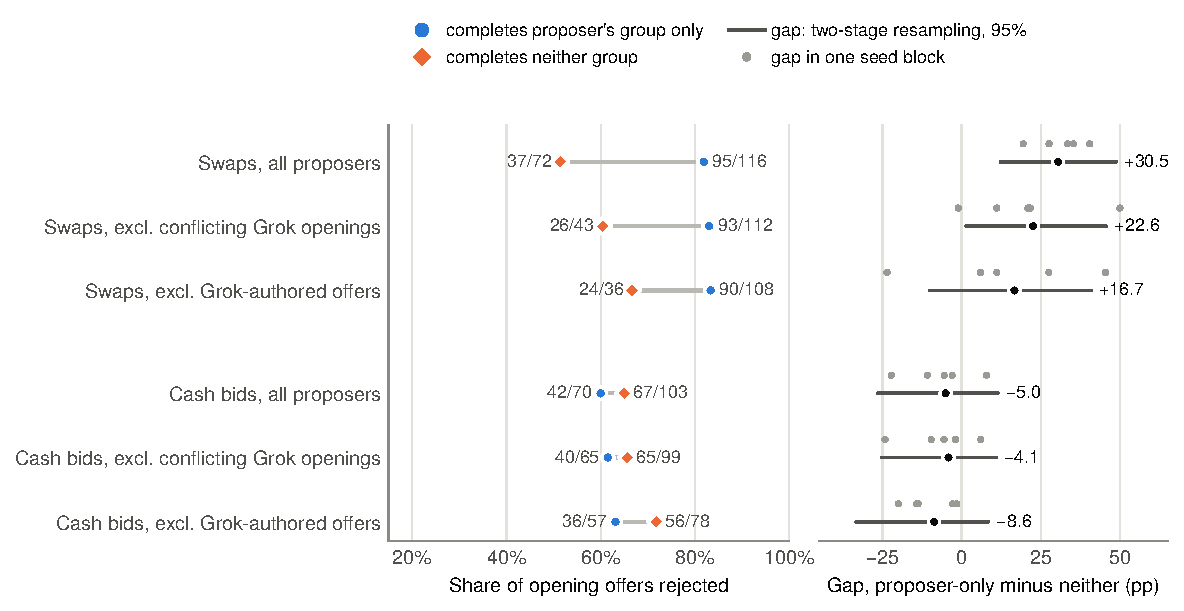
\includegraphics[width=\linewidth]{offer_forms.pdf}
\caption{Opening-offer rejection by form, completion and proposer composition. Left: rejection shares with counts. Right: the gap in percentage points, with the interval from resampling seed blocks and then games within blocks (20,000 draws), and the gap in each seed block shown separately above it. The contrast was selected after inspecting this corpus, so the intervals describe its spread within the cohort and do not confirm it.}
\label{fig:forms}\end{figure}

\subsection{Spread across seed blocks}
Figure~\ref{fig:forms} shows the same comparisons across the five seed blocks. With all offers, the swap gap is positive in every block, from 19.4 to 40.5 points, and dropping any one block leaves 28.7 to 33.3. Without Grok-authored offers it is positive in four blocks; in the fourth, all four remaining comparison swaps are rejected and the gap is $-23.5$. The two-stage resampling interval is $+12.3$ to $+48.8$ points for all swaps, $+1.4$ to $+45.7$ without conflicting openings and $-10.0$ to $+40.9$ without Grok-authored offers. For cash bids it is $-26.5$ to $+11.4$. That interval includes no difference and moderate differences in either direction, so the records do not show that completion is irrelevant to cash bids. Appendix~\ref{app:offers} gives every block and two other resampling units.

\subsection{What recipients say}
Two LLM-assisted readings of an earlier draft coded 74 direct rejections of offers that would complete the \emph{recipient's} own group, 38 recipient-only and 36 completing both parties. They agree that 61 of the 74 cite a trade-linked consequence for the rival. Gemini and Grok supply 56 of the 61, and G1 and G15 supply 31. None of the 74 offers belongs to the proposer-only or neither cells of the form comparison. They show that refusals often state what the rival gains, not why swaps and cash bids differ, and no human validated them.

To look at the comparison cells themselves, we ran a single regular-expression screen over each recipient's public message and applied note (Appendix Table~\ref{tab:keyword}). It is a screen, not a coding. Rejections of proposer-only swaps mention completion in 93 of 95 cases and building in 83; rejections of proposer-only cash bids mention completion in all 42 and building in 35. The stated reasons are much the same under both forms. What differs is the action. Recipients counter 26 of the 70 completing cash bids and 20 of the 116 completing swaps, and 15 of those 26 cash-bid counters keep the same deeds and ask for more cash.

\subsection{Two alternative explanations}
A recipient might simply reject bundles that give it little. Yet at list prices proposer-only swaps offer recipients more than comparison swaps (median net $+\$170$ against $+\$80$). Among swaps that favor the recipient at list prices, 86 of 103 proposer-only swaps are rejected against 24 of 48 comparison swaps, and 81 of 95 against 18 of 25 without Grok's offers. List price omits mortgage status, complementarity and the blocking value of the requested deed. Blocking value is the quantity at issue, so this check narrows the immediate-benefit explanation without removing it.

A recipient might instead track how much the proposer could build next. Rejection of proposer-only swaps does not rise with the proposer's post-trade house budget: 26 of 33 when it could buy one or two houses, 42 of 48 for three to five and 23 of 27 for six or more. Cash bids show no ordering either (Appendix Table~\ref{tab:capacity}). The cells are small and cash omits mortgage capacity, but these slices give no sign that refusals scale with the rival's building power.

The bargaining evidence reaches \Level{stated} for many refusals and \Level{accurate} and \Level{consistent} in individual cases, but not \Level{sensitive}. One description fits the counts: completing the proposer's group is usually met with refusal in a swap and with a higher price in a cash bid. Why is not identified.

\IncidentTitle{g15}{A refusal that cites the rival's building cash}
At G15 turn 63, Sol has \$730 and Grok \$333. Sol offers its two greens for Grok's Ventnor and \$100. The trade would complete Sol's yellows and Grok's greens:
\TranscriptQuote{g15-offer}
Grok's applied note compares what each side could build afterwards:
\TranscriptQuote{g15-refusal-note}
The post-trade cash figures, \$830 and \$233, match the offer ledger. A first green level costs \$600, though a single legal green house costs \$200. Sol drops its cash request, adds Kentucky Avenue, and finally offers both greens, Kentucky and \$250. Grok refuses again:
\TranscriptQuote{g15-final}
All three offers fail. Within twenty turns Grok is bankrupt and its yellow and green blockers pass to Gemini; Sol never completes either group. This incident reaches \Level{accurate} and \Level{consistent}: the refusal states a correct post-trade cash comparison and acts on it. Whether refusing was better than accepting is unknown.
\TranscriptSource{G15 d168--175, standard prompt. Each public message was found in the addressee's next stored prompt.}

\IncidentTitle{g2}{Pricing a deed against the buyer's construction budget}
At G2 turn 45, Opus holds two yellows and bids \$325 for Sol's Marvin Gardens. Sol counters:
\TranscriptQuote{g2-ask}
\TranscriptQuote{g2-ask-note}
One turn earlier Sol had asked Grok, which held no yellow, for \$450 for the same deed. The \$520 remainder is right, but nine yellow houses would cost \$1,350. Sol comes down to \$600 while Opus raises its bid to \$400 and then \$450, writing ``\InlineQuote{g2-final-inline}'' Its note keeps a higher ceiling:
\TranscriptQuote{g2-ceiling}
Sol keeps Marvin Gardens. At turn 69 the positions reverse: Opus, down to \$17, sells Sol its two yellows for two railroads and \$100. Sol builds two yellow houses, sells them four turns later, and loses the group to Gemini at its bankruptcy on turn 86. The ask differs by buyer, and Opus's ``final'' bid is a bluff that fails. The incident reaches \Level{stated} and \Level{consistent}, with an inaccurate building count.
\TranscriptSource{G2 d124--128 and d197--198. Quoted public messages were found in the addressee's next stored prompt. Opus's d127 bid uses the standard prompt; its later sale uses recovery.}

\IncidentTitle{g19}{Correcting a false premise while accepting good terms}
Grok's call offers Virginia Avenue and \$150 for Sol's States Avenue, with this message:
\TranscriptQuote{g19-false}
Both deeds are pink. Grok's own applied note on the same call disagrees, and its assistant content names a different action:
\TranscriptQuote{g19-abort}
\TranscriptQuote{g19-content}
The engine applies the received call, and the proposal reaches Sol, which answers:
\TranscriptQuote{g19-correct}
The trade completes no group, and Sol's note records \emph{``No opponent monopoly enabled.''} Sol separates the factual claim from the terms and evaluates the terms. This reaches \Level{accurate} and \Level{consistent} for Sol. Grok's three channels disagree, so the false message cannot be read as a coherent deceptive plan.
\TranscriptSource{G19 d135--136, standard prompt. Grok's message was found in Sol's d136 prompt; the note and assistant content were not delivered.}
